\chapter[Light Confinement]{Light confinement in sub-wavelength nano-structures} \label{LM}


\section{Light and Nanowire} \label{LightNW}

We have demonstrated that core-shell nanowires grown on Si or GaAs substrate
have extraordinary enhanced optical and electronic properties compared to their
thin film counterparts in the previous chapter. However, the question about how
the light interact with these sub-wavelength structures still remains, and one
cannot simply apply ray-optics to solve this issue. Thus, in this chapter, a
proper model of electromagnetic wave propagation and resonating in the
cavities will be proposed, and the general solutions of this eigen problem will
be discussed. In addition, with the aim of finite-difference-time-domain (FDTD)
simulation, we generalized the volumetric cavity modes in CSNWs, and studied
their geometric dependence and light engineering applications.

\subsection{Modal Analysis of Cylindrical Nanowire}

The general equation describing the scalar wave (e.g., single components of the
electromagnetic field) is:

\begin{equation}
  {\nabla}^2u-\frac{1}{c^2}\frac{{\partial}^2u}{\partial{t}^2}=f(r,t)
\end{equation}

where $u(r,t)\in\mathbb{C}$ is the wave field amplitude, c is the wave speed or
phase velocity, $f(r,t)\in\mathbb{C}$ represents wave field sources. By
applying the technique of separation of variables
$u(r,t)=\psi_\zeta(r)e^{-i\omega_zeta{t}}, Re(\omega_\zeta)\geq0$ (from
$e^{-i\omega_\zeta{t}}=e^{-i\Re(\omega_\zeta)t}e^{-i\Im(\omega_\zeta)t}$ we
observe that solutions with $\Im(\omega_\zeta)\neq0$ dissipate in time as
"leaky modes") to reduce the complexity of the analysis and considering the
free wave equation $f(r,t)\equiv{0}$, we obtain the Helmholtz or the amplitude
wave equations for a nanostructure representing by electromagnetic field:

\begin{equation}
  {\nabla}^2\bm{E} + {\omega}^2\mu\epsilon\bm{E} = 0
\end{equation}
\begin{equation}
  {\nabla}^2\bm{H} + {\omega}^2\mu\epsilon\bm{H} = 0
\end{equation}

where $\bm{E}$ and $\bm{H}$ are the macroscopic electric and magnetic fields,
respectively. This is an eigenvalue equation for the operator $\nabla^2$ with
eigenvalues ${\omega}^2\mu\epsilon$ and eigenfunctions $\bm{E}$ and $\bm{H}$.
Because all other components of both electric and magnetic fields can be
derived from their z component, we only consider $\bm{E}_z$ and $\bm{H}_z$
here,

\begin{equation}
  \frac{{\partial}^2\bm{E}_z}{\partial{r^2}} +\frac{1}{r}\frac{\partial\bm{E}_z}{\partial{r}} +\frac{1}{r^2}\frac{{\partial}^2\bm{E}_z}{\partial{{\phi}^2}} + \frac{{\partial}^2\bm{E}_z}{\partial{z^2}} +{\omega}^2\mu\epsilon\bm{E}_z = 0
\end{equation}
\begin{equation}
  \frac{{\partial}^2\bm{H}_z}{\partial{r^2}} +\frac{1}{r}\frac{\partial\bm{H}_z}{\partial{r}} +\frac{1}{r^2}\frac{{\partial}^2\bm{H}_z}{\partial{{\phi}^2}} + \frac{{\partial}^2\bm{H}_z}{\partial{z^2}} +{\omega}^2\mu\epsilon\bm{H}_z = 0
\end{equation}

Under specified boundary conditions, these equations can only be solved for a
discrete set of eigenfrequencies $\omega_\zeta$ (resonant angular frequencies)
with an index $\zeta$ (also called mode numbers). These special solutions
(called the eigenmodes) allow us 1) to write the general solution of the free
wave equation $(f(r,t)\equiv0)$ as a linear combination of eigenmodes, and 2)
to obtain the solution to the harmonically forced wave equation $(f(r,t) =
F(r)e^{-i\omega{t}})$. The general solutions for the above equations can be
written as,

\begin{equation}
  \bm{E}_z(r,\phi,z)=\psi(r)e^{-j\beta{z}}e^{-jv\phi}
\end{equation}

If at the edge of the cavity, only the wave speed changes, $c_1$ inside the
cavity and $c_0$ outside, and the refractive index inside the cavity defined as
$n=c_0/c_1$, outside the cavity as $1$ for air. We impose the following
boundary conditions: 1) the function $\psi(r)$ should be finite everywhere (no
singularities), 2) it should describe only outgoing waves for
$r\rightarrow\infty$, 3) the wave function should be continuous at the edge of
the cavity at $r=a$.

Thus, we have the wave function inside the cylinder $(r<a)$,
\begin{equation}
  {r^2}\frac{{\partial}^2\psi}{\partial{r^2}}+r\frac{\partial\psi}{\partial{r}}+r^2({k_0}^2n^2-\beta^2-\frac{v^2}{r^2})\psi = 0
\end{equation}
and outside the cylinder $(r>a)$,
\begin{equation}
  {r^2}\frac{{\partial}^2\psi}{\partial{r^2}}+r\frac{\partial\psi}{\partial{r}}+r^2({k_0}^2-\beta^2-\frac{m^2}{r^2})\psi = 0
\end{equation}

where $k_0=\omega_\zeta/c$ is the wave number, and $\beta$ is the wave vector
in z direction. Define $\kappa$ and $\gamma$ as wave vectors in the transverse
direction inside and outside of the cylindrical structure;

\begin{equation}
  \kappa^2={k_0}^2n^2-\beta^2
  \label{eq:kappa}
\end{equation}
\begin{equation}
  \gamma^2={k_0}^2-\beta^2
  \label{eq:gamma}
\end{equation}

After applying the separation of variables in a cylindrical coordinates system
$(r,\varphi)$, the Bessel $J_m$ and Hankel functions ${H_m}^{(1)}$ of the first
kind of order $m$ will be the proper solution for Eqs.~\ref{eq:kappa}
and~\ref{eq:gamma}, respectively:

\begin{equation}
  \psi_\zeta(r)=e^{im\varphi}\cdot\left\{
    \begin{array}{ll}
      A_\zeta\cdot{J_m}(nk_0r)\quad;\quad r<a\\
      B_\zeta\cdot{H_m}^{(1)}(k_0r)\quad;\quad r>a
    \end{array}
    \right.
\end{equation}

The first boundary condition determines the ratio $B_\zeta$ over
$A_\zeta$~(\ref{eq:BAratio}) and the second one determines the eigenfrequency
$\omega_\zeta$ from the characteristic equations~(\ref{eq:characterEq}), which
can only be solved numerically due to its transcendental form. Thus,

\begin{equation}
  \frac{B_\zeta}{A_\zeta}=\frac{J_m(nk_0a)}{{H_m}^{(1)}(nk_0a)}
  \label{eq:BAratio}
\end{equation}
\begin{equation}
  \frac{{J_m}^\prime(nk_0a)}{{J_m}(nk_0a)}=\frac{1}{n}\cdot\frac{{H_m}^{(1)\prime}(nk_0a)}{{H_m}^{(1)}(nk_0a)}
  \label{eq:characterEq}
\end{equation}

where the prime denotes ordinary differentiation.

To be more specific, the excitation of leaky modes occurs in an infinitely-long
dielectric cylinders of radius $a$ when the following condition is satisfied;
i.e., the characteristic equation is~\cite{Cao:2009ho}:

\begin{equation}
  {(\frac{1}{\kappa^2}-\frac{1}{\gamma^2})}^2{(\frac{\beta{m}}{a})}^2={k_0}^2(n^2\frac{{J^\prime}_m(\kappa{a})}{\kappa{J_m}(\kappa{a})}-{n_0}^2\frac{{H^\prime}_m(\gamma{a})}{\gamma{H_m}(\gamma{a})})(\frac{{J^\prime}_m(\kappa{a})}{\kappa{J_m}(\kappa{a})}-\frac{{H^\prime}_m(\gamma{a})}{\gamma{H_m}(\gamma{a})})
  \label{eq:LMcharacter}
\end{equation}

Equation~\ref{eq:LMcharacter} can be split in conditions for purely transverse
magnetic (TM) modes, if a cylinder in vacuum and air $(n_0=1)$ is illuminated
by normal incidence $(\beta=0)$, with the magnetic fields in the plane normal
to the nanowire axis
$[n{J^\prime}_m(nK_0a)/J_m(nk_0a)={H^\prime}_m(K_0a)/H_m(k_0a)]$ and transverse
electric (TE) modes
$[{J^\prime}_m(nK_0a)/nJ_m(nk_0a)={H^\prime}_m(K_0a)/H_m(k_0a)]$ with the
electric fields normal to the nanowire axis. From these conditions it follows
that nanowires tend to support a limited number of TE and TM leaky modes, which
increase in number as their radius is increased. Detailed discussion of Leaky
Resonant Mode will be present in the following section~\ref{sec:LMR}.

On the other hand, Whispering Gallery Modes (WGM) can also be supported by
solving the characteristic equation~\ref{eq:characterEq} numerically. They
correspond to waves circling around the cavity, supported by continuous total
internal reflection off the cavity surface, and return to the same point with
the same phase after round trip, thus, interfere constructively with
themselves, forming standing waves.

One of the most important quantities that describe the performance of any
resonator is the quality factor or Q-factor. It can be defined
as~\cite{tobing2010fundamental}:

\begin{equation}
  Q=\omega_0 \frac{Stored\ energy}{Power\ loss}=\omega_0\tau=\frac{\omega_0}{\triangle\omega_{FWHM}}=\frac{\Re(\omega_\zeta)}{2|\Im(\omega_\zeta)|}
  \label{eq:Qfactor}
\end{equation}

where $\omega_0=2\pi{v_0}$ is the angular frequency and $v_0$ is the frequency
of the resonance, $\tau$ is the cavity ring down lifetime (i.e., the time
required for the field intensity to decay by a factor of e) and
$\triangle\omega_{FWHM}={\tau}^{-1}$ is the linewidth of the frequency of the
resonance in angular frequency.

Large Q-factors are necessary for most applications. The Q-factor measures the
characteristic time for the natural decay of the energy stored inside the
resonator in terms of the number of full field oscillations (times $2\pi$).
This means that for a higher Q-factor the time that energy is stored inside the
resonator is proportionally longer, and the total field intensity of the
resonating mode will be higher 

The last term in Eq.~\ref{eq:Qfactor} express the Q-factor of the resonance
mode from the complex propagation constant (wave number):
$k_0=\frac{\omega_\zeta}{c_0}=\beta+\frac{1}{2}i\alpha$, where
$\beta=\frac{2\pi}{\lambda_0}=\Re(\omega_\zeta)$ is the phase constant,
$\lambda_0$ is the wavelength in vacuum or air, and
$|\alpha|=2|\Im(\omega_\zeta)|$ is the intensity attenuation coefficient due to
various cavity loss mechanisms.

\subsection{Leaky Mode Resonance}
\label{sec:LMR}

Interaction of light with a dielectric or metallic cylindrical medium is
analyzed by solving Maxwell's equations with the appropriate boundary
conditions in the classical waveguide theory~\cite{Kapany2012optical}, which
leads to highly confined modes in optical fibers and microscale dielectric
resonators.  In an infinitely long cylinder, even at deep sub-wavelength
diameters this results in a “characteristic equation~\ref{eq:LMcharacter},” the
solution to which are the transverse magnetic (TM) and transverse electric (TE)
resonant modes. We can define the electromagnetic modes of localized resonators
as time-harmonic solutions of the form $\bm{E}(\bm{r},t) =
\bm{E}(\bm{r},\omega)e^{-i\omega{t}}$ to the source-free Maxwell equations.
This solution shows that the longitudinal field component distributes outside
the NW and is in resonance with the natural modes, such as ${TE}_{11}$,
${TM}_{02}$, etc., supported by the NW.  These modes have been termed
leaky-mode resonances (LMR)~\cite{Cao:2009ho,Fountaine:2014de}, and provide an
intuitive tool to facilitate the understanding and optimization of the
resonance effect in such nano-structures.

In order to gain an understanding of light confinement and guiding in NWs. We
replicate previous results using MEEP, a widely used open-source
finite-difference time-domain (FDTD) simulation package~\cite{Oskooi:2010fb},
to identify how light is confined in an infinitely long GaAs nanowire. The top
row of Fig.~\ref{CylindEz} shows several configurations of TM LMR modes for a
NW with diameter of 220 nm, with excitation single wavelength light being
incident parallel to the NW axis. The blue and red color codes represent the
polarization of the electric fields. The TE modes are primarily identical to
the TM modes shown here with the electric and magnetic fields exchanged. If the
light is incident with an arbitrary angle, then so-called hybrid HE and EH
leaky modes will be excited instead of the pure TE or TM mode. The bottom row
of Fig.~\ref{CylindEz} shows the directional energy flux density of the
electromagnetic field, the Poynting vector, at different time frames with light
being incident perpendicular to the NW axis from the right side. The light is
seen to propagate from the right and then mostly remain confined at the left
part of the cylinder. It is notable that in either case the light energy is
spatially distributed along the cross section of the wire but, as expected from
a 2D treatment does not vary axially. Figure~\ref{CylindEz} demonstrates that
the LMR can gently confine light within subwavelength semiconductor
nano-structures, similar to the intuitive ray-optics picture of multiple total
internal reflections from the periphery of the cylinder. As shown by in
Ref.~\cite{Cao:2009ho}, these LMRs depend on the radius and the height of the
dielectric, which allows ‘light engineering’ of the nanowires so as to increase
its absorption efficiency at pre-determined wavelength, e.g., to maximize
absorption of sunlight spectrum for higher efficiency solar cells, or to
radiate as optical antennas.

\begin{figure}
  \caption{(Top) Resonant modes in an infinitely long cylinder of GaAs with diameter of 220 nm with light incident parallel to NW axis. (Bottom) The Poynting vector at different time frames with light incident perpendicular to the NW axis from the right. The black lines show the physical boundary between the nanowire and air.}
  \centering
  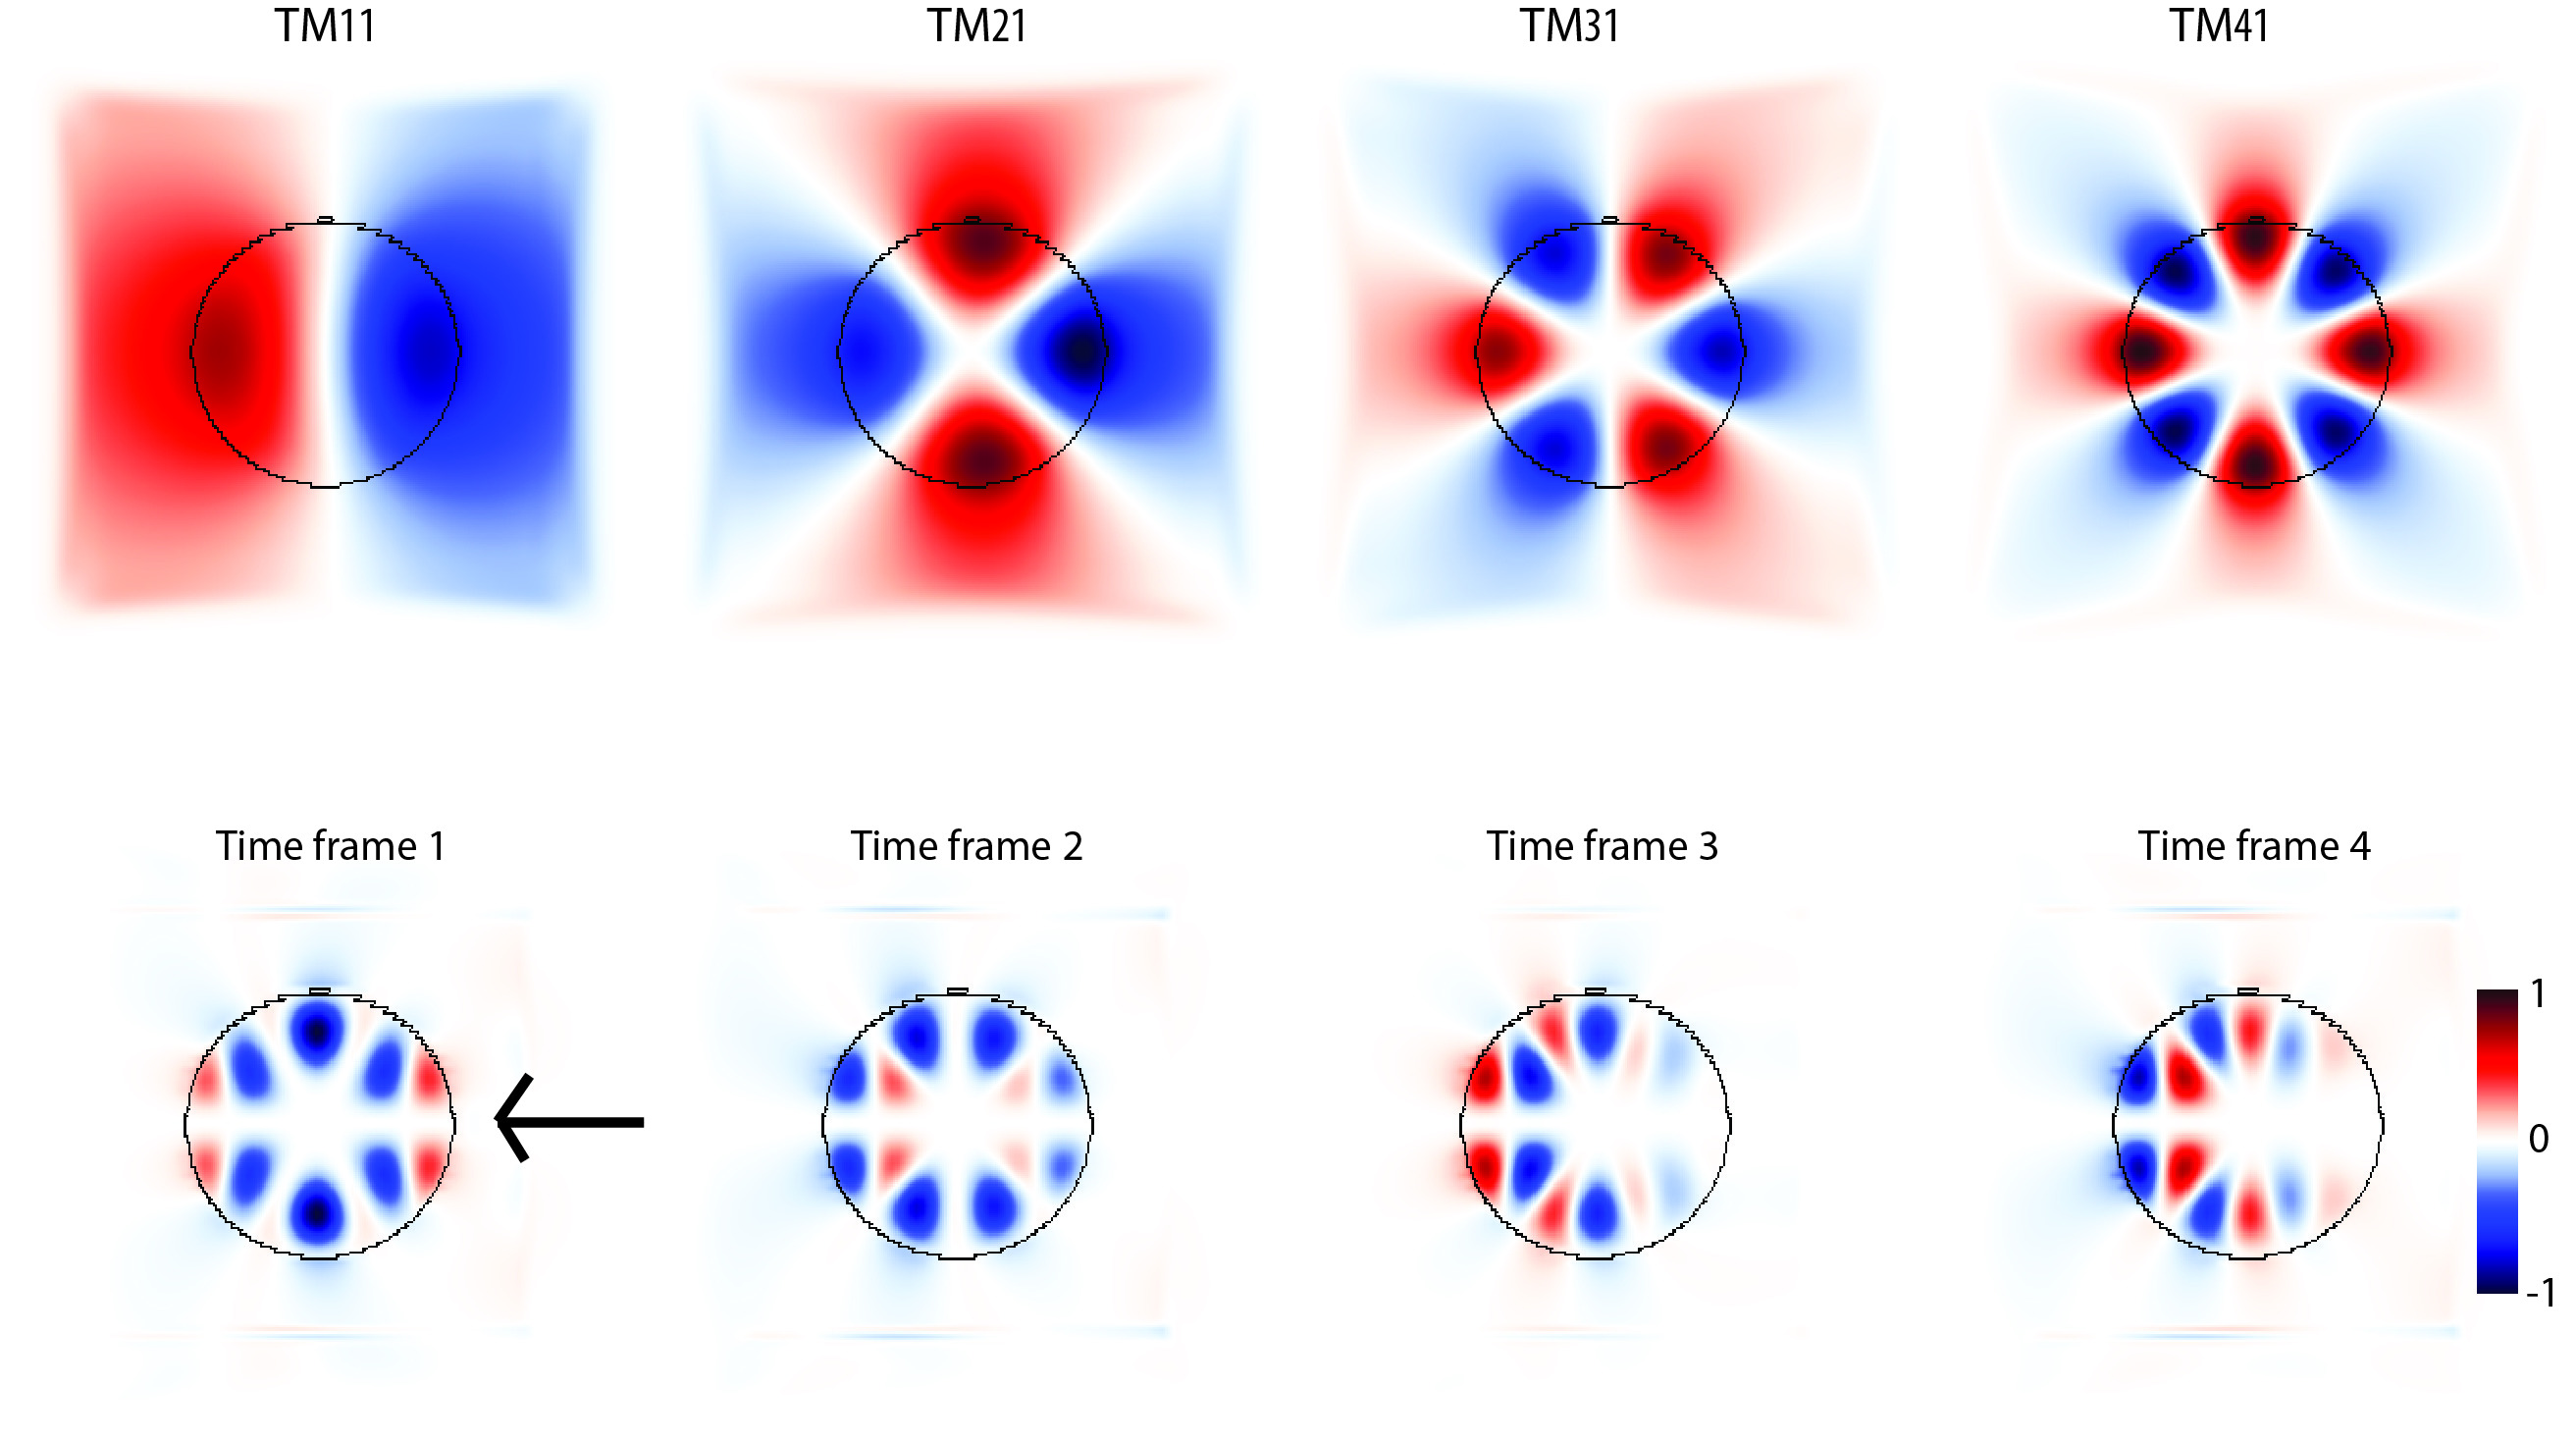
\includegraphics[width=\textwidth]{pictures/LM/CylindEz}
  \label{CylindEz}
\end{figure}

\subsection{Whispering Gallery Modes}
\label{sec:WGM}

Infinitely long cylindrical or hexagonal NW structures can also support
Whispering Gallery (WG)
modes~\cite{Zimmler:2008fc,huang2001room,Zhao:2014jt,Nobis:2005wg,Czekalla:2010uw,Gargas:2009cx,Fallert:2008ej,Johnson:2002ua,Nobis:2004tp}.
To calculate the resonant WGMs, Maxwell's equations have to be solved
numerically~\cite{Wiersig:2003vo} taking into consideration the spectral
dependence of the material of interest's index of refraction. However, we can
deduce a simple plane-wave model from theoretical derivations, and the
relationship between resonance wavelength $\lambda$ and the corresponding mode
serial number N can be obtained~\cite{Nobis:2004tp}. The WG modes can also
reflect and confine light in the (subwavelength) nanostructure by total
internal reflection from the curvature of the structure boundaries. However, a
light wave can interfere with itself only when having completed one full
circulation within the resonator, which means only the light with one or
multiple wavelengths are allowed to perform multiple circulations generating a
standing wave. Figure~\ref{WGMode} from reference~\cite{Nobis:2005wg} shows
near-field intensity patterns of low-order TM polarized hexagonal WGMs for $n =
1$ and refractive index $n_r = 2.1$. Each mode pattern is labeled by its
respective mode number m (lower right number) and its symmetry class (upper
right symbol).

For comparison, four mode patterns of the circular cavity are given in the
upper left and lower right together with their angular mode number. We again
observe the radial spatial dependence of light intensity. Furthermore, the low
order WG modes of hexagonal NWs are essentially similar to the cylindrical
ones, but for higher order modes additional features will arise on the facets
of the hexagonal NWs~\cite{Nobis:2005wg}. Simulation results also show little
difference between WG mode and Leaky modes in lower order modes for both
hexagonal and cylindrical structures. As with the LMR, the resonant WG modes
have been used as the basis for a precise theoretical explanation of the
enhanced optical behavior of hexagonal NWs, such as enhanced light
absorption~\cite{Cao:2009ho,Kim:2014ig,Zhang:2013wb,Kelzenberg:2010fa,Wang:2013ux}
and emission~\cite{Zimmler:2008fc,Currie:2013to,Le:2014cp,Grzela:2012wa}.
Furthermore, these numerical solutions have lead to reproduction of
experimental resonance spectra, e.g., polarization-resolved
micro-photoluminescence $(\mu-PL)$ and cathodeluminescence (CL) spectroscopy.

\begin{figure}
  \caption[Several configuration of Whispering Gallery resonance modes in infinite long cylindrical and hexagonal nanowires.]{Several configurations of Whispering Gallery resonance modes in infinite long cylindrical and hexagonal nanowires. For comparison, four mode patterns of the circular cavity are given in the upper and lower right together with their angular mode number. (Reprinted with permission from~\cite{Nobis:2005wg} , \textcopyright 2005 by the American Physical Society.)}
  \centering
  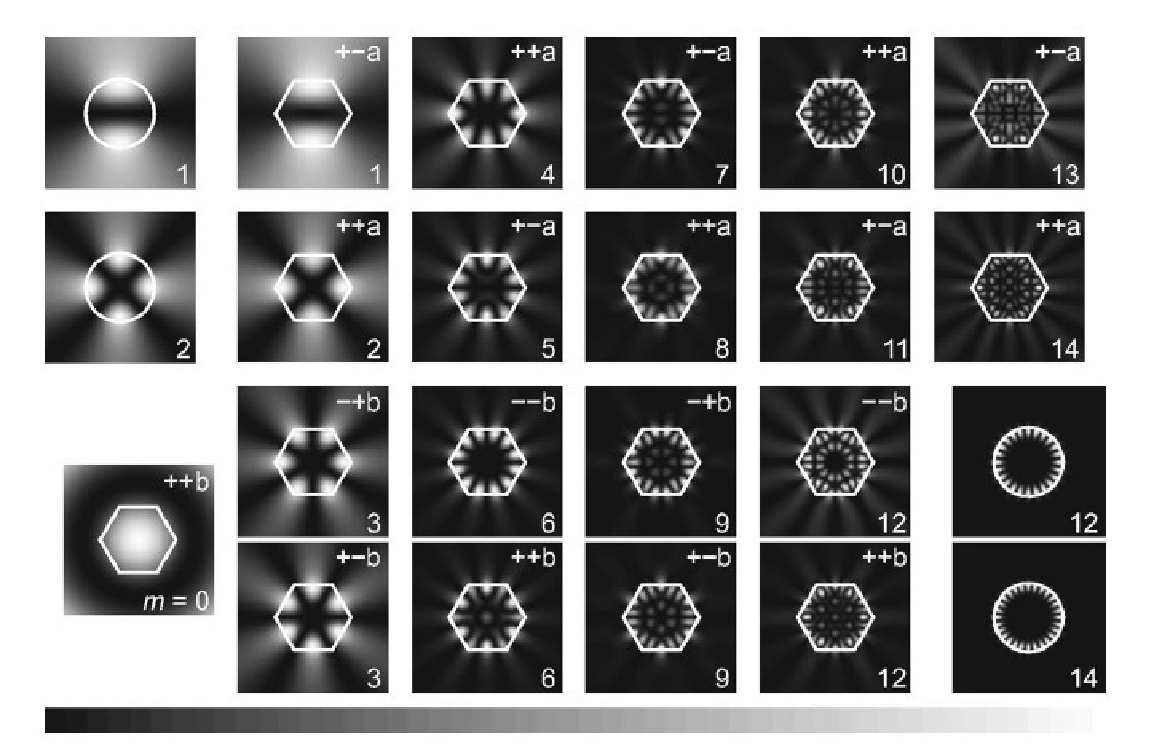
\includegraphics[width=\textwidth]{pictures/LM/WGMode}
  \label{WGMode}
\end{figure}

\subsection{Fabry-P{\'e}rot Resonant Mode}

The above analysis and results apply to long structures, hence, provide
two-dimensional radial modes, independent of the NW axis. However, light
confinement has strong axial dependence, necessitating three-dimensional
analysis of the cavity modes. FDTD simulation in 3D are used to identify the
axial dependence of resonant modes in these nano-structures, revealing modes
which are volumetric in nature.

Fabry-P{\'e}rot (FP) modes have been analyzed for sub-microcavity, or nano-cavity,
NWs with cylindrical or hexagonal structures, specifically in order to
determine the axial dependence of the resonance modes ~\cite{Maslov:2003cq}. At
least two mirrors are needed to construct the reflection structure inside the
cavity, whether they are the top and bottom ends, i.e., the air and substrate
interfaces with the nanowire, or any of the two opposite facets along the
nanowire axis. For subwavelength structures, the longitudinal WG modes have
high scattering losses due to diffraction, and axial FP waveguide modes will
dominate~\cite{Johnson:2002ua}. However, due to small difference of the
refractive index between the substrate and the nanowire dielectric, the
existence of the FP mode will only be valid if the nanowire has relatively
large radii, e.g., larger than 200 nm~\cite{Hua:2007fn}. Under these
conditions, besides the top and bottom ends, the lateral facets of nanowire can
also be treated as two parallel slabs, and with the dielectric in between, it
can support the FP mode with mode spacing inversely related to the nanowire
length. An application of this analysis is in the design of NW lasers, since
the optical cavity modes are observed at threshold for lasing, and have been
investigated for both optical and electrical pumped cases
~\cite{Duan:2003en,Saxena:2015cn}. As a results the FP resonance mode based
nanoscale lasers are not only capable of covering a wide spectral regions, but
can also can be integrated as single or multi-color laser source arrays in
silicon based photonic integrated circuit or microelectronic devices
~\cite{Duan:2003en,Saxena:2015cn}. However, the FP modes supported by the
nano-cavity structure have relatively small quality factor due to the small
difference of the refractive indices of the substrate and the NWs. In order to
address this issue, Bragg gratings can be produced at the NW ends,
alternatively, NWs can be placed on metal substrates in order to increase the
FP resonance peak intensity by more than one order of magnitude compared to
those on Si substrates~\cite{Arab:2014wy}.

\subsection{Helical Resonance Modes}

Nanoneedles of III-V material grown on heterogeneous substrates are
optoelectronic devices which have shown interesting optical behavior, including
lasing, at room temperature~\cite{Chen:2011cg}. Figure~\ref{HelicalMode} (a)
shows SEM image of a nano-laser grown on silicon substrate that has
subwavelength dimensions on all sides. Analysis of light propagation shows that
unlike the traditional WG mode that lack vertical structure, there is net
propagation in axial direction in these structures which leads to volumetric
resonant modes which are termed helical mode resonances~\cite{Chen:2011cg}. The
schematic Fig.~\ref{HelicalMode}(b) suggests a helical ray path with nearly
total internal reflection at the nanopillar-silicon interface due to the
glancing angle of incidence from the hexagonal facets of the nano-laser shown
in Fig.~\ref{HelicalMode}(a). As such, the faceted shape of the structure
affects the optical cavity properties. FDTD-simulated field profile shows a
hexagonal WG-like mode pattern  in the transverse plane as in
Fig.~\ref{HelicalMode} (c), which arises from strong azimuthal components of
helical modes.  Figure~\ref{HelicalMode} (d) shows first-order and higher-order
standing waves’ axial variation. The radial mode number (first number, m)
describes the transverse field pattern for WG modes, and the axial mode number
(second number, n) describes the axial standing wave as is the case for
Fabry-Perot resonances. It is seen that light or optical field can be well
confined in the nanostructure even with low index contrast at the dielectric
interface thus producing the nano-resonators needed for lasing. Although the
quality (Q) factors of such nanostructure are usually not large, these
helically propagating cavity modes, provide an optical feedback mechanism
without the sophisticated mirror structures of the vertical cavity surface
emitting lasers (VCSEL's). Additionally, since the nanowires are
heteroepitaxially grown on different substrates, they enable heterogeneous
integration of photonic emitters and silicon based computational circuitry.
Whereas traditional FP modes are inhibited by the interface between
semiconductor nanostructure and the silicon substrate, such unique optical
structures have been proposed as an avenue for engineering and integrating
on-chip nanophotonic devices.

\begin{figure}
  \caption[Hexlically propagating modes for optical feedback.]{Helically propagating modes for optical feedback. (a) SEM image of the nanolaser grown on silicon substrate. (b) Schematic depicting a helical ray path because of glancing angle of incidence from the hexagonal facetes of the nanolaser shown in (a). (c) FDTD-simulated field profile shows a hexagonal WG-like mode pattern in the transverse plane, which arises from strong azimuthal components of helical resonance modes. (d) First-order and higher-order standing waves' axial variation. (Reprinted with permission from Macmillan Publishers Ltd: Nature Photonics~\cite{Chen:2011cg}, \textcopyright2011)}
  \centering
  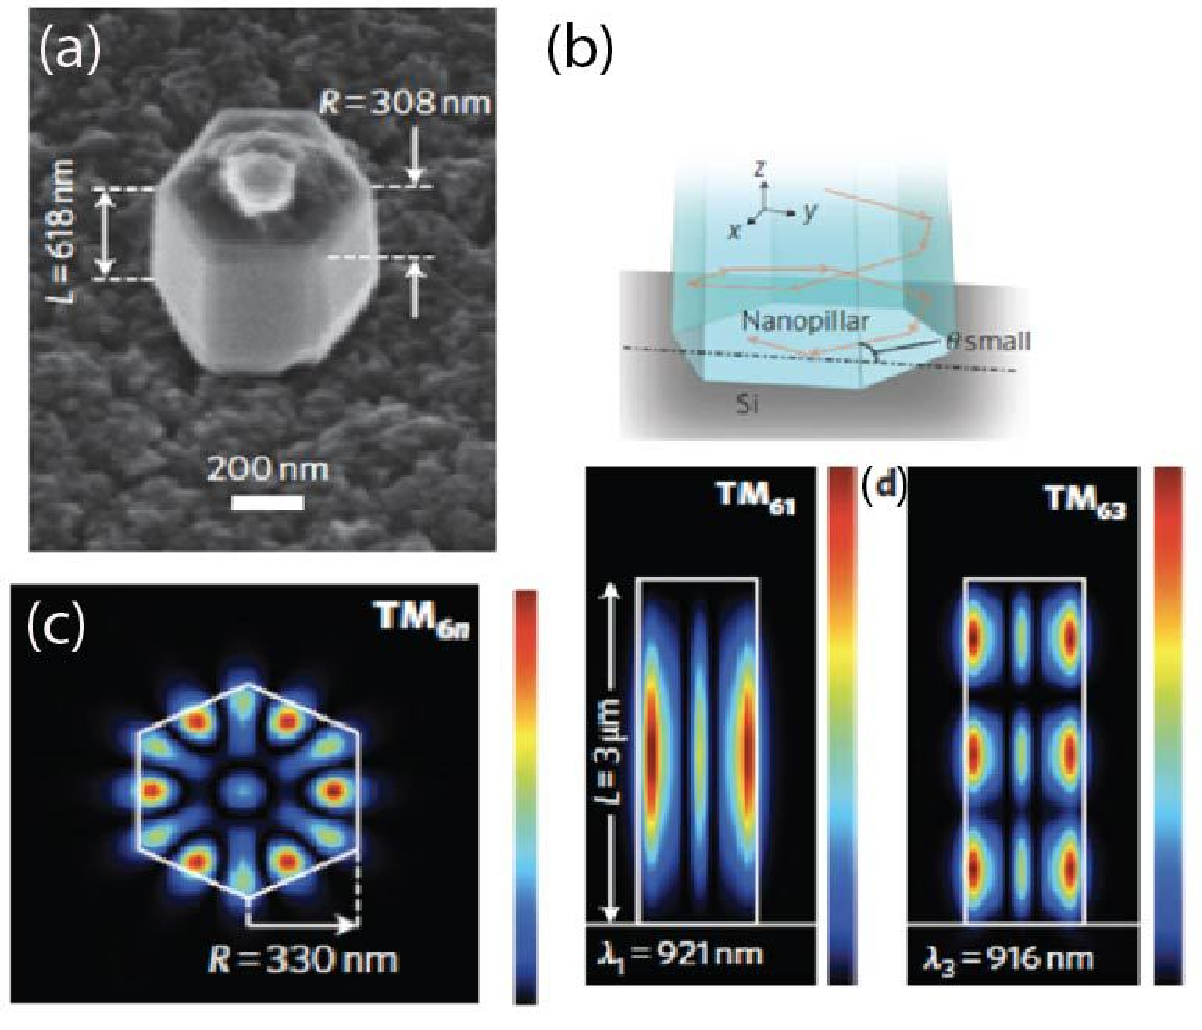
\includegraphics[width=\textwidth]{pictures/LM/HelicalMode}
  \label{HelicalMode}
\end{figure}

\section{Volumetric Modes} \label{VM} 
\subsection{FDTD Simulation}

The finite-difference time-domain (FDTD) algorithm is one of the most common
computational tools in classical electromagnetism, which divides space and time
into a regular grid and simulates the time evolution of Maxwell's
equations~\cite{sullivan2013electromagnetic,taflove2005computational}. The
starting point for any FDTD solver is the time-derivative parts of Maxwell's
equations, which in their simplest form can be written:

\begin{equation}
  \frac{\partial\bm{B}}{\partial{t}} = - \nabla \times \bm{E} - \bm{J}_B
\end{equation}
\begin{equation}
  \frac{\partial\bm{D}}{\partial{t}} = + \nabla \times \bm{H} - \bm{J}
\end{equation}

where $\bm{E}$ and $\bm{H}$ are the macroscopic electric and magnetic fields,
respectively. $\bm{D}$ and $\bm{B}$ are the electric displacement and magnetic
induction fields~\cite{jackson1999classical}, respectively. $\bm{J}$ is the
electric-charge current density, and $\bm{J}_b$ is a fictitious magnetic-charge
current density which is used for the calculation convenience of magnetic-dipole
sources. In time-domain calculations, one typically solves the initial-value
problem where the fields and currents are zero for $t < 0$, and then nonzero
values evolve in response to some currents $\bm{J}(\bm{x},t)$ and/or
$\bm{J}_b(\bm{x},t)$. However,the frequency-domain solver assumes a time
dependence of $e^{-i\omega{t}}$ for all currents and fields, and solves the
resulting linear equations for the steady-state response or
eigen-modes~\cite{joannopoulos2011photonic}.

In this chapter, all the simulation work were carried out by an open-source
simulation package MEEP (an acronym for MIT Electromagnetic Equation
Propagation)~\cite{Oskooi:2010fb}, which implemented the FDTD algorithm. The
advantages of MEEP compared to other commercially available FDTD software
packages are: free and open-source which extends the flexibility provided by
access to the source code. In addition, MEEP is full-featured, including:
arbitrary anisotropic, nonliear, and dispersive electric and magnetic media; a
variety of boundary conditions including symmetries and perfectly matched
layers (PML); distributed-memory parallelism; Cartesian (1d/2d/3d) and
cylindrical coordinates; and flexible output and field computations.

In order to perform the simulation in 2D by MEEP, a core-shell hexagonal
structure has to be constructed using cylindrical coordinates as in
Fig.~\ref{MeepSchematic}, which takes the advantages of geometric symmetries to
reduce the computation time. The radius of AlGaAs shell is 185 nm, and the
radius of GaAs core is 40\% of the shell, i.e., 74 nm. The dielectric constant
for GaAs and AlGaAs sets to be 3.4 and 3.3, respectively. Air with unit
dielectric constant fills between this hexagonal structure and the perfectly
matched layer (PML). The PML is an artificial absorbing layer used to truncate
computational regions with open boundaries for solving electromagnetic wave
equations numerically. The primary difference between PML and an ordinary
absorbing materials is that the waves incident upon the PML from a non-PML
medium do not reflect at the interface, thus, allow the PML to completely
absorb outgoing waves from the interior of a computational region without
reflecting them back into the inner region. Finally, a Gaussian pulse source
at the right corner of the hexagon with certain center frequency and bandwidth
is used to excite the structure. The simulation stops until the sources are
finished, and then to run for some additional period of time. In that
additional period, the electromagnetic field is processed at a specific point
to identify the frequencies and decay rates of the modes that are excited.

3D simulation can be easily performed by adding one additional degree of
freedom which is the nanowire length. The simulated cylindrical and hexagonal
structures with cylindrical coordinates are sketched at the bottom of
Fig.~\ref{NWsketch} (a). The top row of Fig.~\ref{NWsketch} (a) shows the
transverse plane mode for cylindrical (left) and hexagonal (right) core-only NW
which is a cross-section cut at the center of the wire. The middle row depicts
the longitudinal plane mode for cylindrical and hexagonal structures. These
results are transverse magnetic (TM) resonance modes adapted from a single time
frame of the electromagnetic evolving in the NW structure with respect to time.
Figure~\ref{NWsketch} (b) shows the 3D view of electromagnetic field
distribution at the middle of a hexagonal NW. The electrical field is tightly
confined at the corners and facets of the structure with a little light at the
core.

\begin{figure}
  \caption{A schematic illustration of Finite-Difference-Time-Domain (FDTD) Simulation Set Up.}
  \centering
  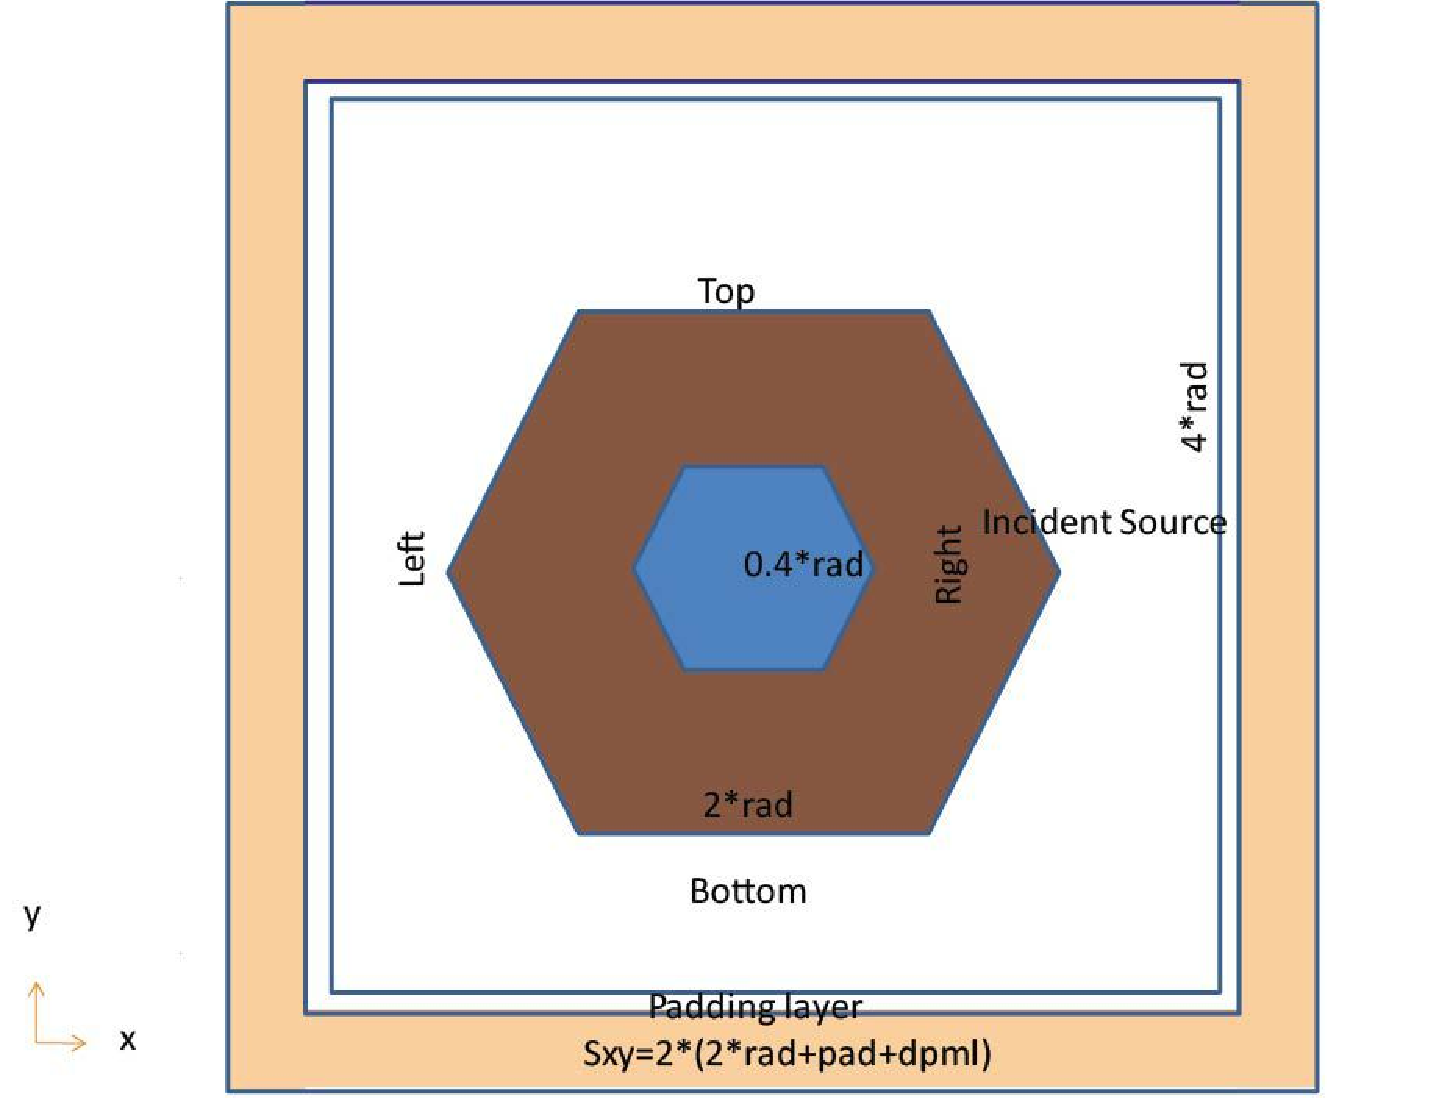
\includegraphics[width=\textwidth]{pictures/LM/MeepSchematic}
  \label{MeepSchematic}
\end{figure}

\begin{figure}
  \caption{(a) (top) Transverse plane mode for cylindrical and hexagonal core-only nanowire. (middle) The corresponding longitudinal plane mode. (bottom) Three dimensional simulation schematic for cylindrical and hexagonal nanowires. (b) 3D view of electromagnetic field distribution at the middle of a hexagonal NW.}
  \centering
  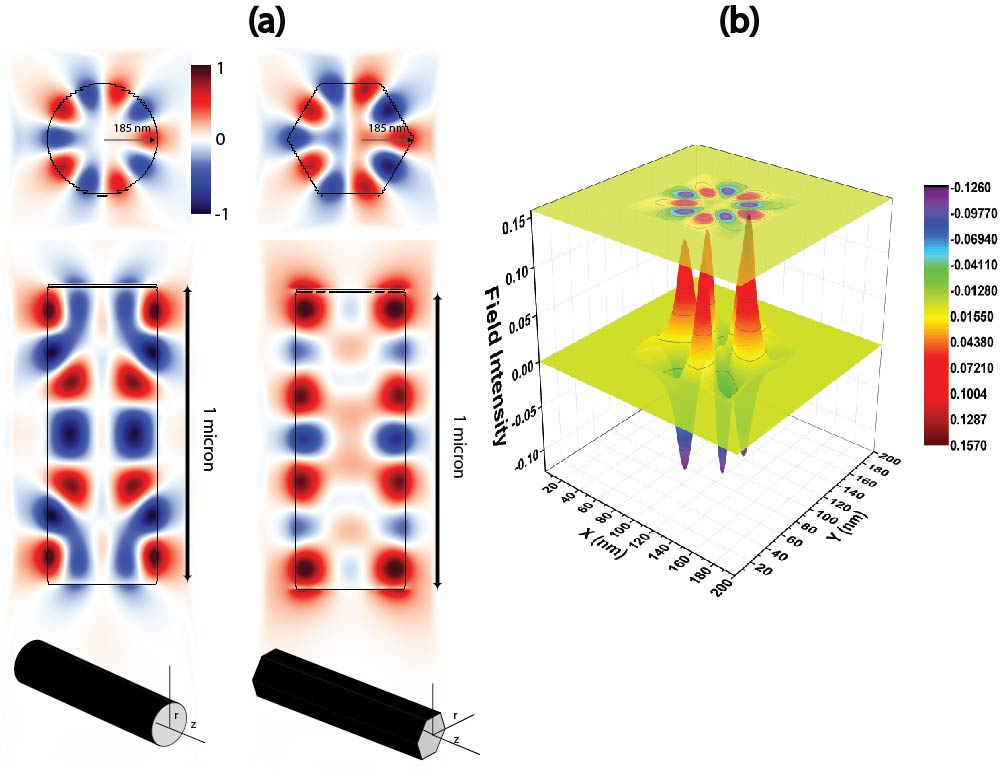
\includegraphics[width=\textwidth,height=0.7\textheight]{pictures/LM/NWsketch}
  \label{NWsketch}
\end{figure}

\subsection{Generalized Volumetric Modes}

The diameter of the nanostructures which can support the helical resonance
modes is near the Rayleigh limit, around the boundary of the validity of
ray-optics. FDTD analysis can be applied to deeper subwavelength structure in
order to identify the cavity modes which are by nature volumetric, i.e.,
axially dependent. Figure~\ref{TMRadiusVarition} shows simulation results for
various diameters of hexagonal structure of 1~$\mu{m}$ length. Incident
radiation with 532 nm wavelength is nearly parallel to the wire axis and
different modes are displayed for different radii. Top row shows radial spatial
dependence at the middle of the wire axis, and the bottom row shows the axial
dependence. Top row results are similar to Figures~\ref{CylindEz} and
\ref{WGMode}, and the bottom row shows that the light can be confined in
volumetric resonance mode in both transverse plane and longitudinal plane even
with sub-wavelength diameter of these hexagonal NWs. Unlike helical modes, the
explanation of resonance need not rely on an intuitive ray-optics description
based on the grazing angle of incident light, but shows similar results in how
the deep subwavelength structures can confine the light and produce a resonant
cavity without having sophisticated mirrors at the end facets. In this respect
nano-cavities of as-grown nanowires outperform microcavities of VCSELs.

\begin{figure}
  \caption{Volumetric cavity modes' dependence on nanowire diameter. Top row is a radial cut at the middle of the wire, bottom row is the corresponding axial spatial variation.}
  \centering
  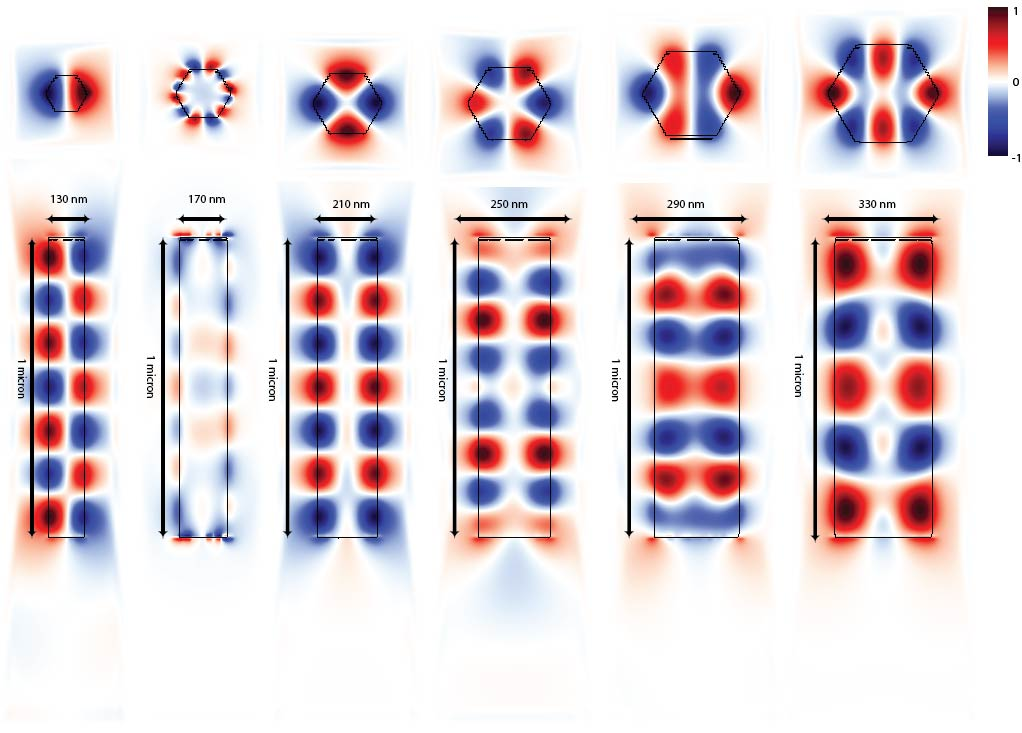
\includegraphics[width=\textwidth]{pictures/LM/TMRadiusVarition}
  \label{TMRadiusVarition}
\end{figure}

The same results that are obtained from hexagonal NWs apply to cylindrical ones
as shown in Figure~\ref{structuredep}, which compares the simulation results
for cylindrical and hexagonal core-only and core-shell NWs with cylindrical
coordinates \(\mathbf{r}\), \(\mathbf{z}\). Since these nano-cavities
resonances have net propagation in the axial direction, two distinct mode
numbers m and n, such as in \(\ \text{TM}_{m,n}\), are used to describe the
azimuthal mode and axial mode, respectively. The transverse magnetic resonant
mode\(\ \text{TM}_{5,7}\) with electric field perpendicular to the nanowire
axis is shown for circular (Fig.~\ref{structuredep} (a), (b)) and hexagonal
(Fig.~\ref{structuredep} (c), (d)) cross-sections. Top row of
Fig.~\ref{structuredep} are the radial standing wave patterns taken at the
middle of the NW, and bottom parts are the axial variation which together
demonstrate standing wave patterns in the nano-cavity. The hexagonal and
cylindrical NWs present nearly identical optical behavior if the nanowires have
the same cross-sectional area, consistent with previous
findings~\cite{Henneghien:2009te}. These simulations produce the same results
as the two-dimensional analysis of Leaky Modes and Whispering Gallery, as well
as the volumetric analysis presented in terms of Fabry-Perot and Helical
resonance modes. The results indicate, however, that there is no need for light
to reflect from the parallel facets of the wire as in the last two
descriptions, rather, the curved surfaces in the sub-wavelength structure can
confine the light equally well.

\begin{figure}
  \caption{Cavity modes for (a) core-only cylindrical, (b) core-shell cylindrical, (c) hexagonal core-only, and (d) hexagonal core-shell. The radius of nanowire is 185 nm and the height is 1~$\mu{m}$.}
  \centering
  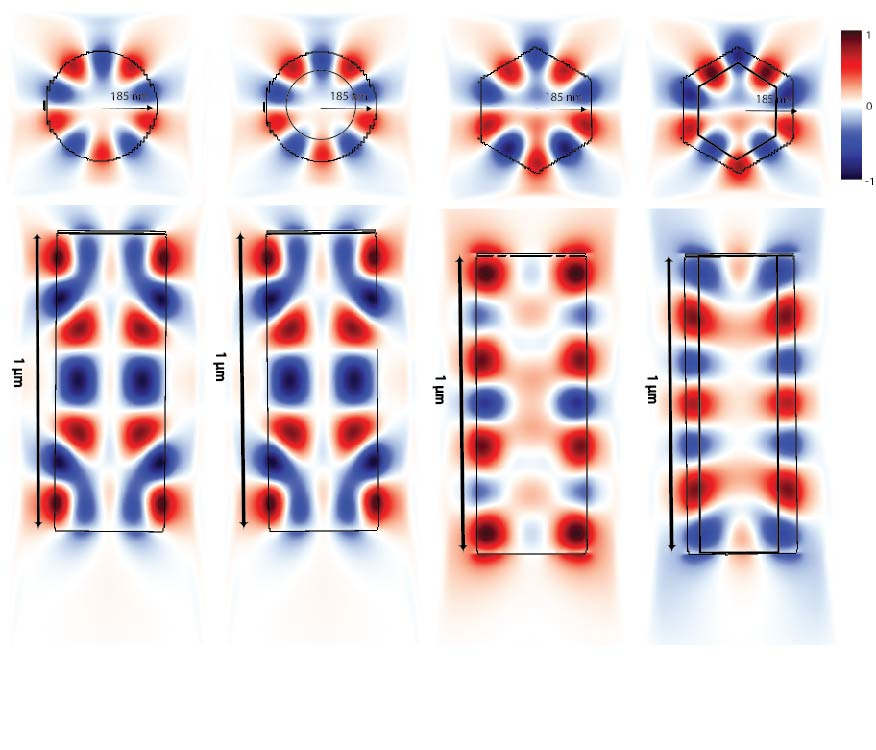
\includegraphics[width=\textwidth]{pictures/LM/structuredep}
  \label{structuredep}
\end{figure}

\subsection{Geometry Dependence of Resonant Modes}

We examine the optical properties of CSNW to see whether it significantly
differs from core-only or dielectric core NWs. Both the materials and the
geometric parameters of the core-shell nanowires can be controlled by the
chemical compositions and/or the temperature/reaction rates during the growth
process. Figure~\ref{CylinRP} and~\ref{HexRP} show the FDTD simulation results
for both transverse plane and longitudinal plane modes for cylindrical and
hexagonal CSNWs at same wavelength (532 nm) of incident light, respectively.
The left part of Fig.~\ref{CylinRP} and~\ref{HexRP} is air-core/AlGaAs-shell,
while the right part is GaAs-core/AlGaAs-shell. And they vary with different
core/shell radius ratios, i.e., (top) $r_{core} = 40\%\ r_{shell}$ (middle)
$r_{core} = 60\%\ r_{shell}$ and (bottom) $r_{core} = 80\%\ r_{shell}$. As
expected, a core with unit dielectric constant will confine the light more into
the shell. The reduction of the shell thickness will further move the light
into the shell with a little light in the core. However, in the right part of
Fig.~\ref{CylinRP} and~\ref{HexRP}, the results clear indicated that the
increasing of the core-shell radius ratio does not modify the electromagnetic
field distribution inside of the CSNWs. The transverse plane modes keep the
same mode number, as ${TM}_{5n}$, for different ratios. In addition, the
materials variation does not alter the mechanisms of confinement of light in
the CSNWs, but only a shift of the resonance frequency corresponding to the
dielectric constant and the bandgap of the materials.

\begin{figure}
  \caption{FDTD simulation results for different ratios, (top) $r_{core} = 40\%\ r_{shell}$ (middle) $r_{core} = 60\%\ r_{shell}$ and (bottom) $r_{core} = 80\%\ r_{shell}$, of core-shell radius of (left) air-core/AlGaAs-shell (right) GaAs-core/AlGaAs-shell cylindrical nanowires.}
  \centering
  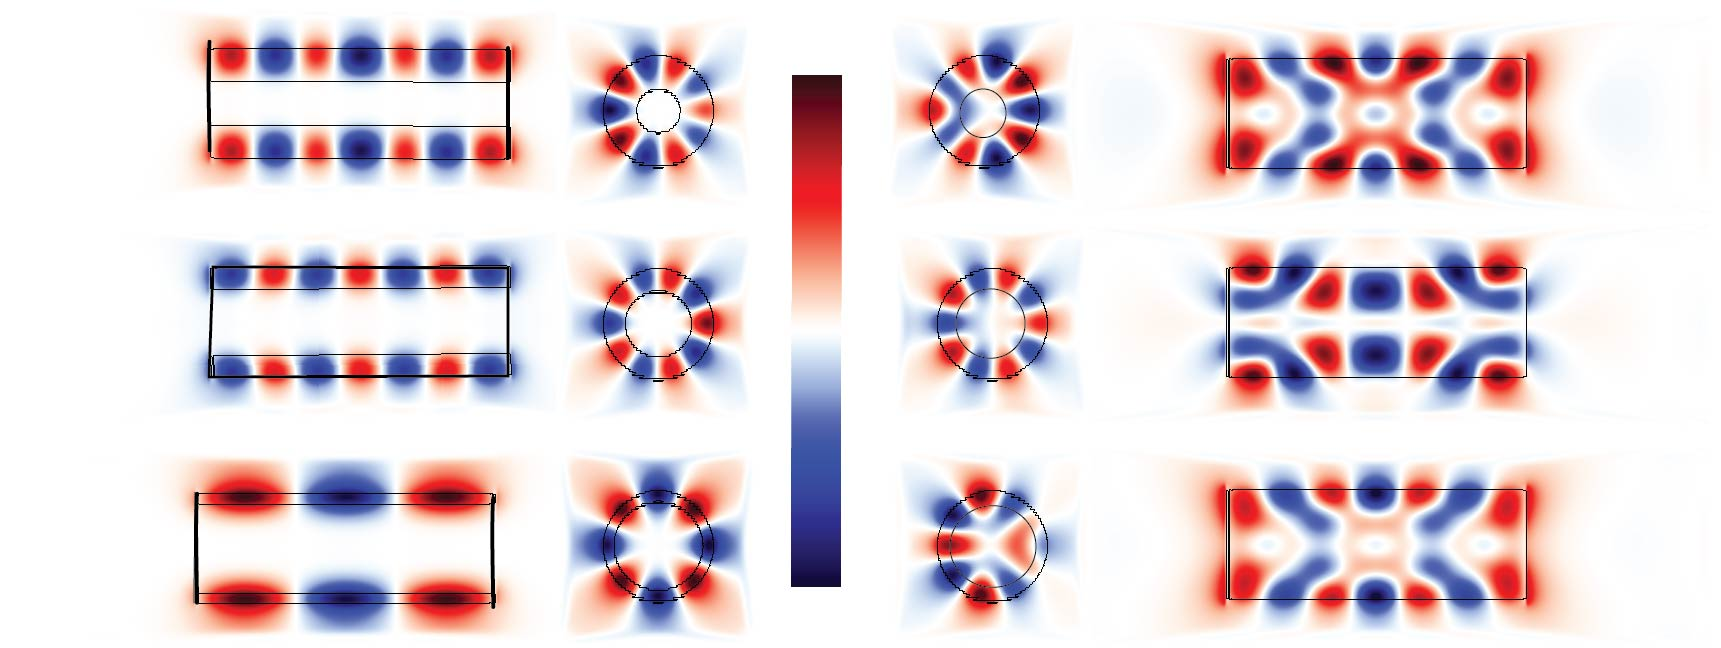
\includegraphics[width=\textwidth]{pictures/LM/CylinRP}
  \label{CylinRP}
\end{figure}

\begin{figure}
  \caption{FDTD simulation results for different ratios, (top) $r_{core} = 40\%\ r_{shell}$ (middle) $r_{core} = 60\%\ r_{shell}$ and (bottom) $r_{core} = 80\%\ r_{shell}$, of core-shell radius of (left) air-core/AlGaAs-shell (right) GaAs-core/AlGaAs-shell hexagonal nanowires.}
  \centering
  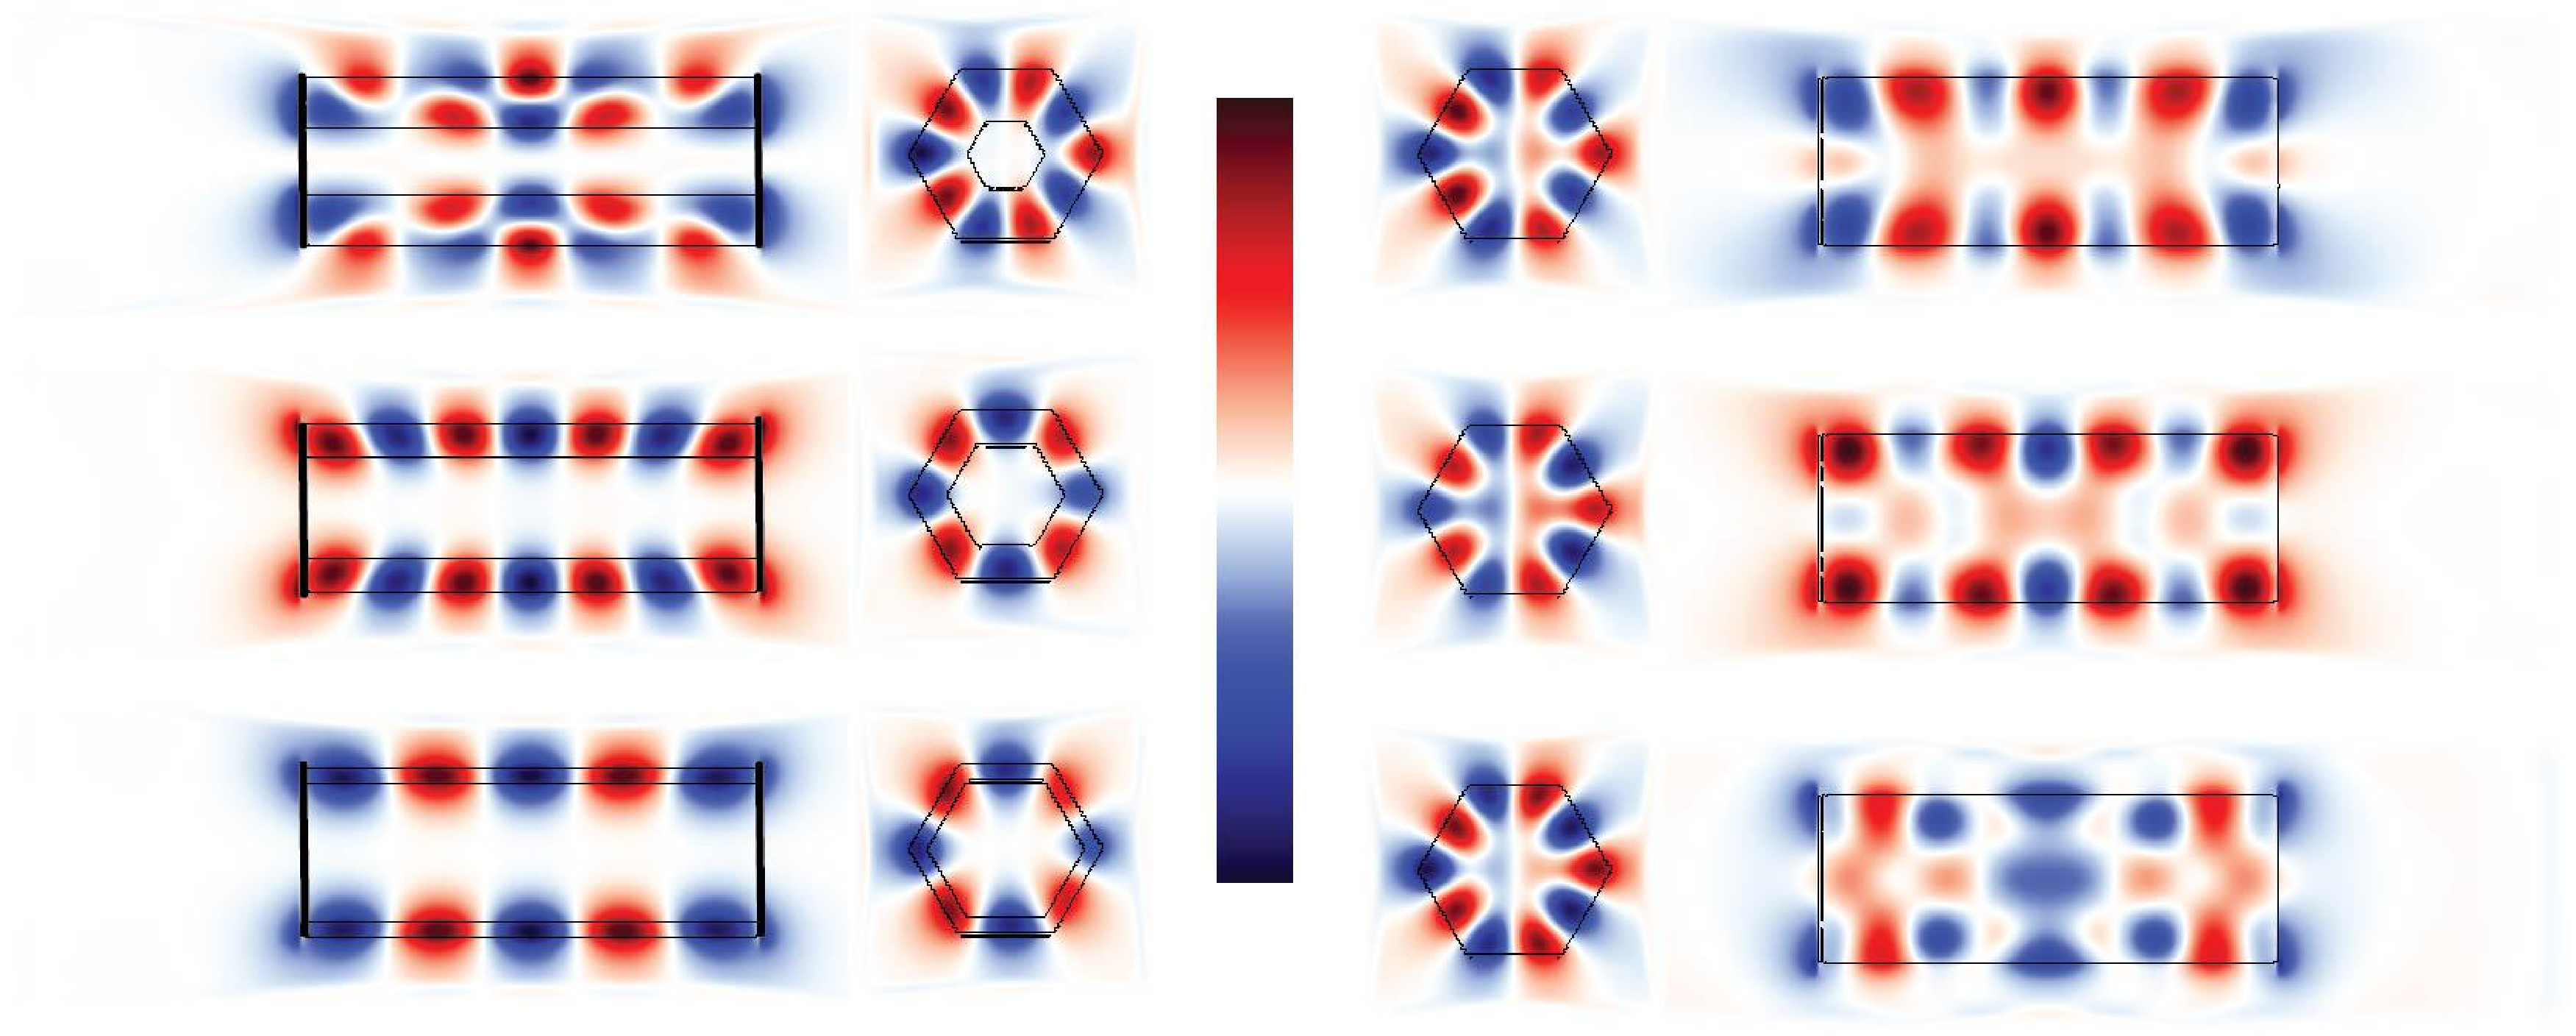
\includegraphics[width=\textwidth]{pictures/LM/HexRP}
  \label{HexRP}
\end{figure}

In Fig.~\ref{TMRadius}, the diameters and the length dependence of the CSNWs
have been studied. The top two rows are transverse plane TM modes with
diameters varying from 20 nm to 370 nm at same wavelength (532 nm) of incident
light. Bottom row is the longitudinal plane TM modes with length varying from
$0.5 \mu{m}$ to $3 \mu{m}$ while remain the same diameters. The results
demonstrated that with increasing of the diameters or lengths while remain the
other factor same, the resonant mode numbers also increased correspondingly.
However, if the diameter of the CSNW is smaller than 150 nm, there is no clear
confined resonant modes excited by the structure which is consistent with the
findings in Ref.~\cite{Zimmler:2008fc}.

\begin{figure}
  \caption{Geometric Dependence TM radius variation for different diameters and length. Top two rows are the transverse plane TM modes with diameters varying from 20 nm to 370 nm. Bottom row is the longitudinal plane TM modes with length varying from $0.5 \mu{m}$ to $3 \mu{m}$.}
  \centering
  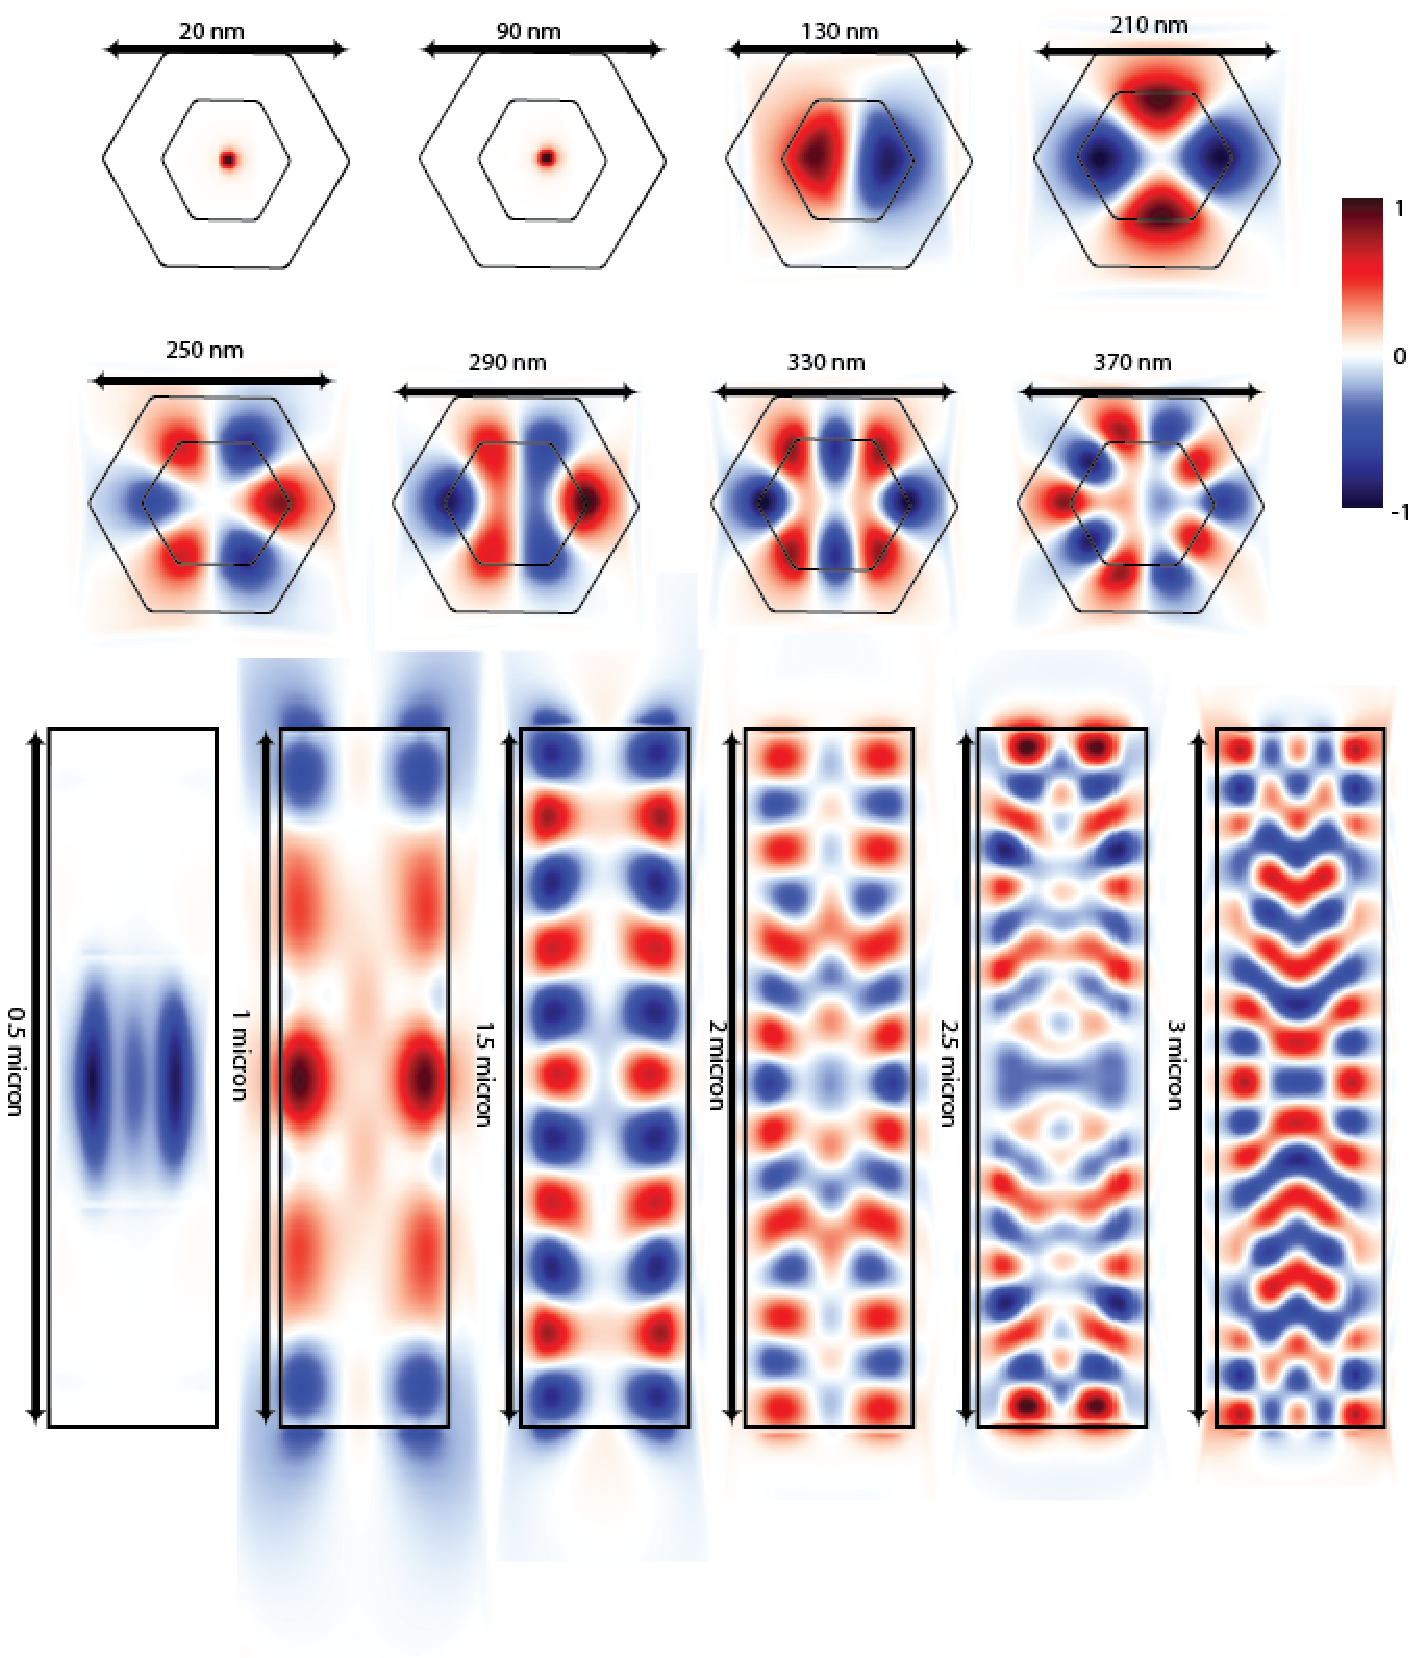
\includegraphics[width=\textwidth]{pictures/LM/TMRadius}
  \label{TMRadius}
\end{figure}

Additionally, figures~\ref{structuredep}(b) and~\ref{structuredep}(d) show
simulation of cylindrical and hexagonal structures, respectively, with core of
GaAs and shell of AlGaAs. These simulations show that there is little
difference between core-only as in Fig.~\ref{structuredep} (a, c) and
core-shell (b, d) NWs, since the difference of the refractive indices of core
and shell is small. Despite being optically identical, these structures have
very different optoelectronic properties which will be discussed in
Chapter~\ref{RM} after describing the important ramifications of the optical
analysis of NWs.

\subsection{Light Engineering of sub-wavelength Nano-structure}

Dependence of the resonant modes on the cavity geometry offers an important
degree of freedom to engineer a cavity for particular optical properties.
Figure~\ref{TMRadiusScat} shows the dependence of three volumetric TM resonant
modes’ excitation wavelengths with radius. In this spectral range, only lower
TM modes can be excited with smaller radii, e.g., r = 40 nm and 60 nm, however,
as the radius increases, higher order modes can be excited, and the optical
power corresponding to the lower order modes will be reduced. We observe
redshift of these volumetric TM modes with increasing NW radius. Also, the
wavelength variation of ${TM}_{1n}$ mode is much larger compared to ${TM}_{2n}$
and ${TM}_{3n}$ modes. These observations demonstrate the feasibility to
engineer the volumetric mode at certain wavelength, i.e., allow us to optimize
absorption or emission at a desired frequency or certain incident optical power
by controlling the radius and/or length of a NW thus providing the ability to
engineer the absorption spectrum in order to match desired properties.

\begin{figure}
  \caption{Correlation of the volumetric TM modes' excitation wavelength with NW radius allows optimization of cavity for absorption and emission at desired wavelengths.}
  \centering
  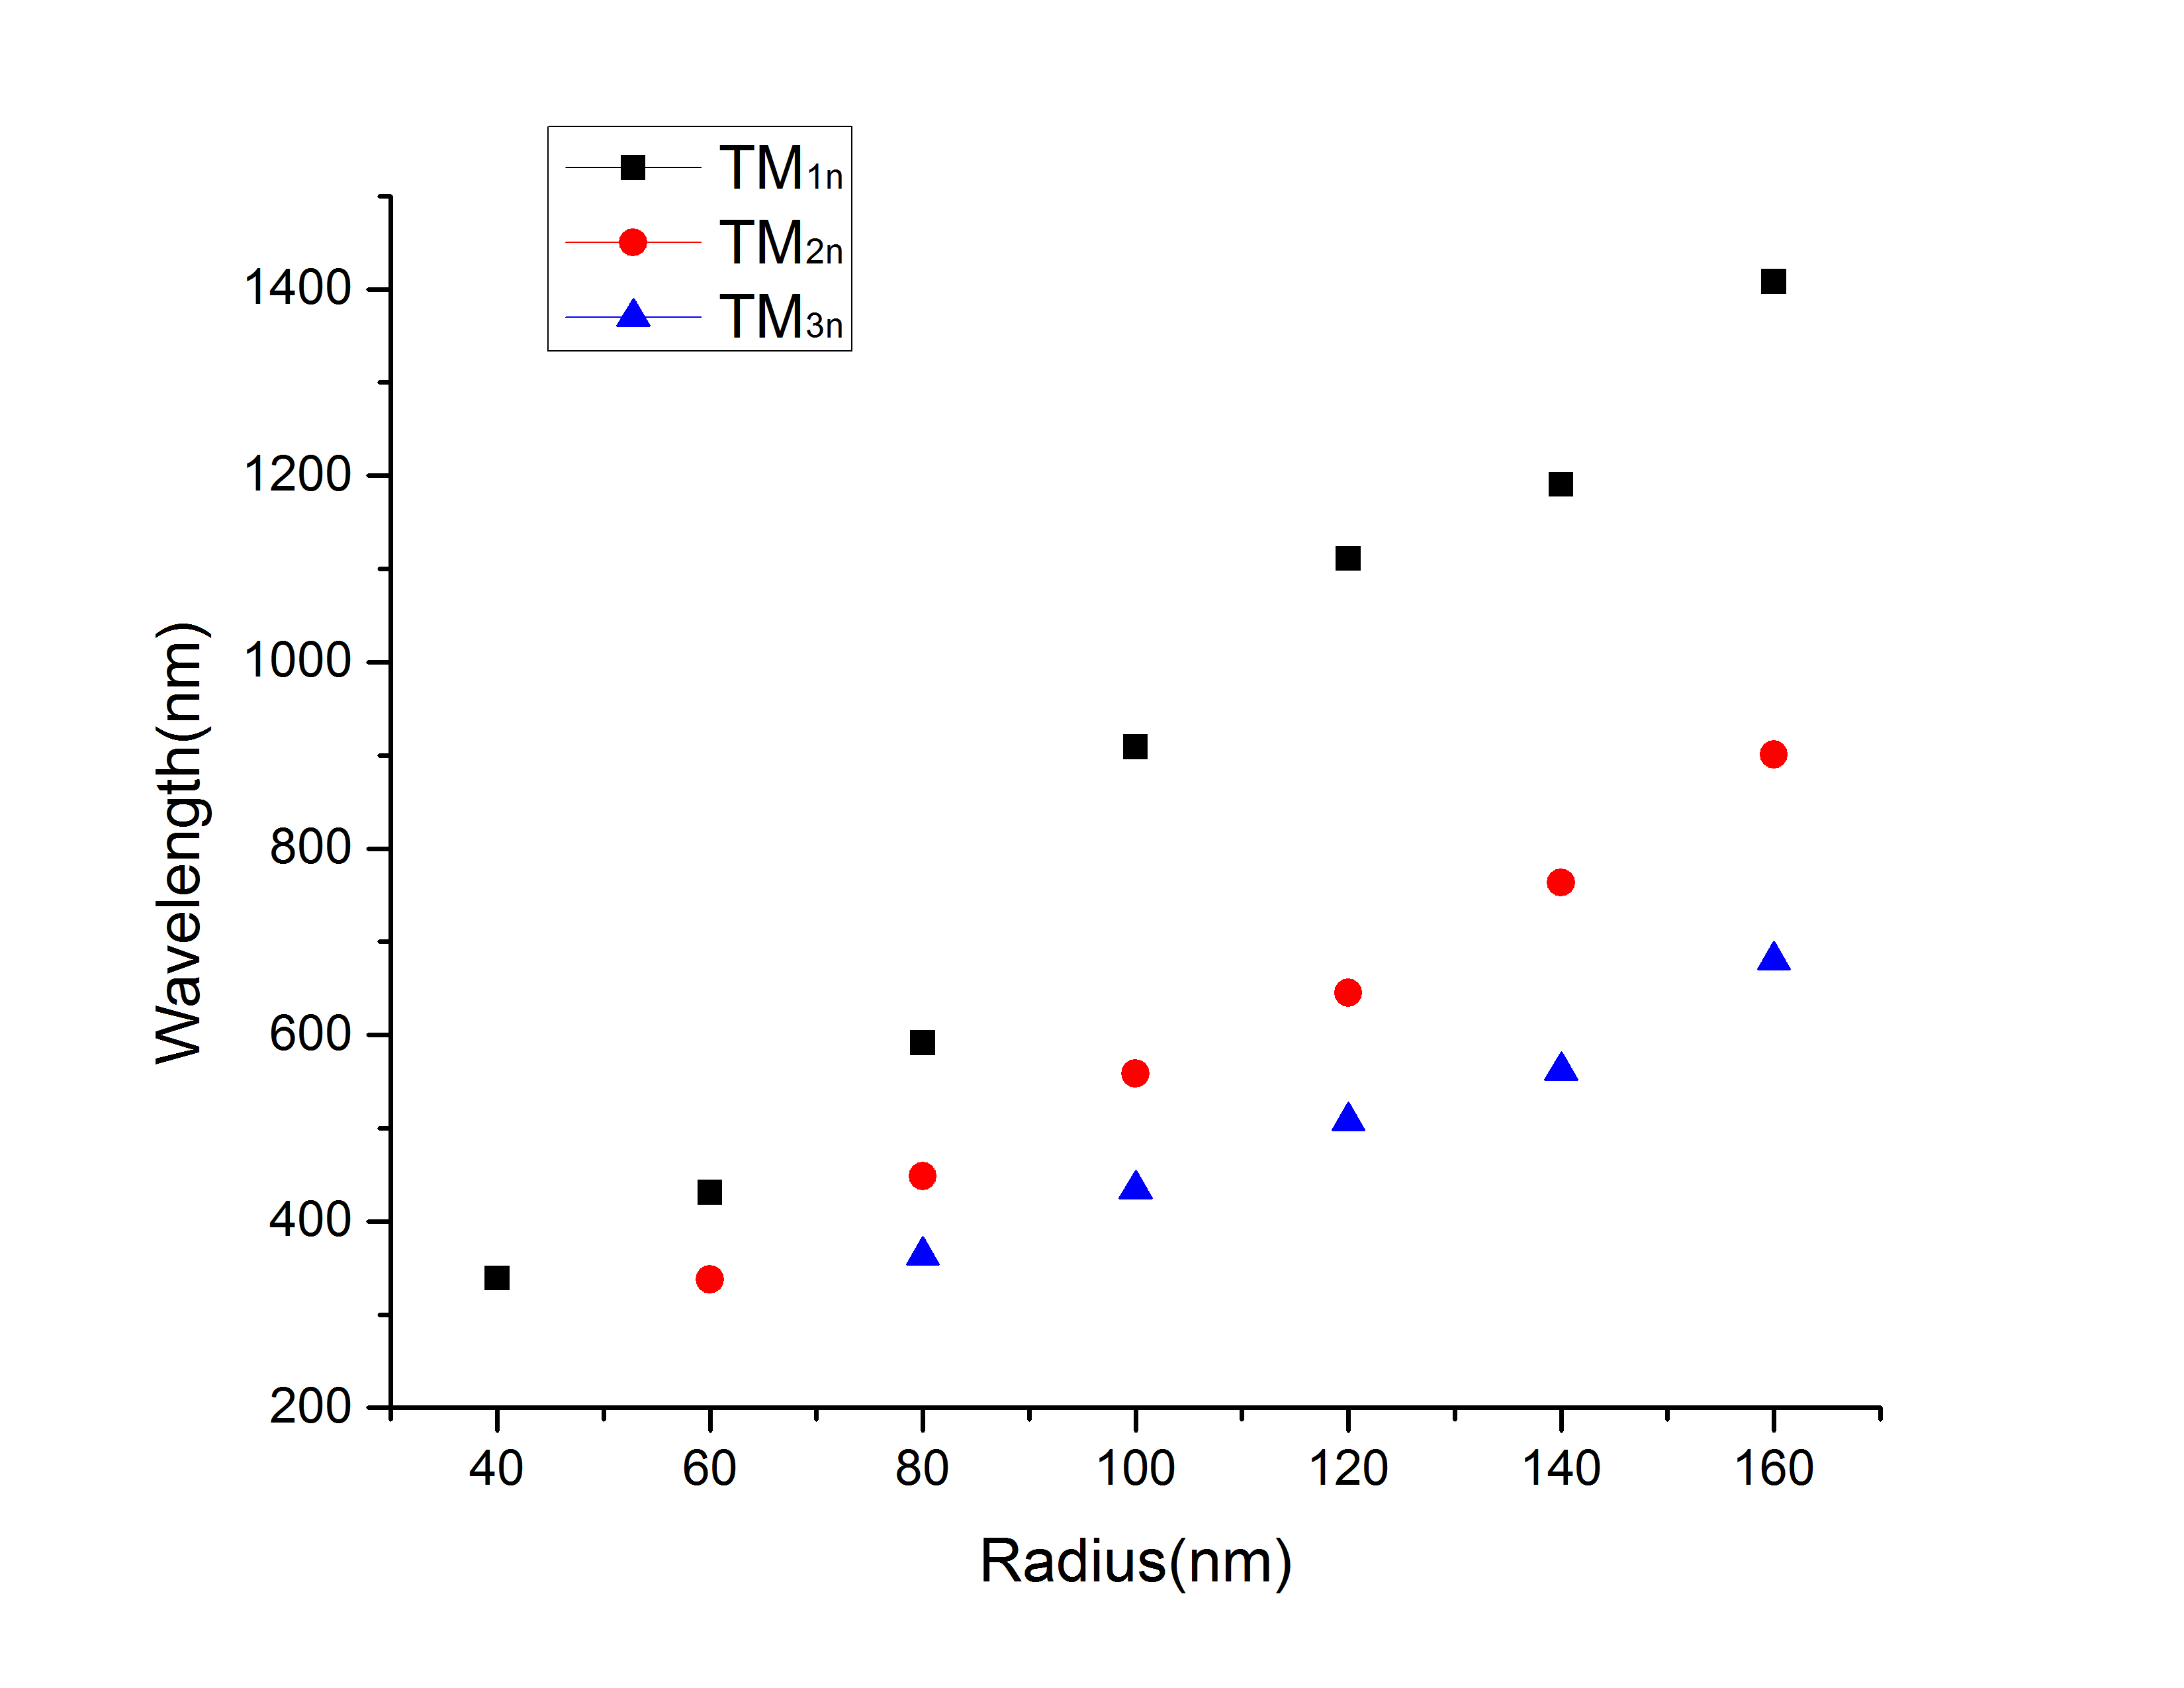
\includegraphics[width=\textwidth]{pictures/LM/TMRadiusScat}
  \label{TMRadiusScat}
\end{figure}

\subsection{Continuous Variation of Geometry - The Tapering effect}

The dependence of the resonant modes on NW radius also suggests the
interesting possibility of having tapered structures which can support more
than one resonant mode, thus be able to optimize the spectrum of interest. The
metalorganic vapor phase epitaxy (MOVPE) or vapor liquid solid (VLS) growth
methods are readily capable of forming nanowires with tapered sidewalls. The
resultant cavity, however, does not support the superposition of the modes
present in cylindrical structures of the same diameter; in fact tapered
sidewalls have been identified as the primary loss mechanism for these
sub-wavelength cavities.

The effect of tapering has been studied for hexagonal CSNW that were grown on a
silicon substrate with average $5^{\circ}$ angles between opposite sidewalls;
vertical electrical field intensity $({|E|}^2)$ profiles for (a) ${TM}_{61}$
and (b) ${TM}_{62}$ modes under different excitation wavelength are shown in
Fig.~\ref{Tapering}, which similar to the result in Ref.~\cite{Chen:2011cg}.
Figure~\ref{Tapering} (c, d) show first-order and higher-order transverse plane
modes at different positions along the wire growth axis. The modes are
primarily confined at the base, and become less resonant as they propagate
upwards with decreasing of the radius at top. Higher-order axial modes
generally have lower quality factor.  Physically, the stronger Fabry-Perot
characteristic of higher-order axial modes means that their effective
longitudinal wave-vector components become stronger, causing larger penetration
and loss into the substrate. Nevertheless, from a different perspective,
multi-mode resonances can be achieved within certain wavelength range by
controlling the tapering angle in order to form small varying radius along the
nanostructure axial direction as in Fig.~\ref{Tapering} (c, d). One can also
red- or blue-shift the resonance peaks, since these volumetric resonance modes
are dependent on transverse dimensions. Thus, intentioned tapering offers an
alternative way to engineering the multi-mode resonances and finer tunability
of these resonance peaks.

\begin{figure}
  \caption{FDTD simulated electric field intensity distribution $({|E|}^2)$ of hexagonal core-shell nanowire on top of Si substrate with $5^{\circ}$ tapering effect. (a, b) field intensity distribution along axial direction with different incident light wavelength, (c, d) field intensity distribution in the transverse plane at different positions along the NW.}
  \centering
  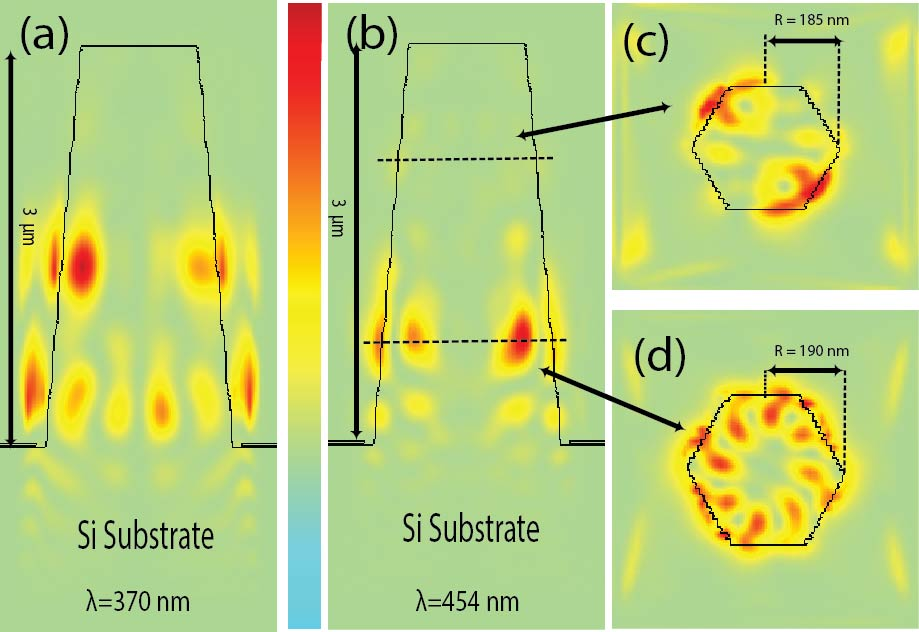
\includegraphics[width=\textwidth]{pictures/LM/Tapering}
  \label{Tapering}
\end{figure}
